\documentclass[12pt]{article}

\usepackage{amsmath}
\usepackage{amsfonts}
\usepackage{graphicx}
\usepackage{amsthm}
\usepackage{algpseudocode}

\usepackage{fancyvrb}
\DefineShortVerb{\|}

\setlength{\oddsidemargin}{0in}
\setlength{\textwidth}{6.5in}
\setlength{\topmargin}{0in}
\setlength{\headheight}{0in}
\setlength{\headsep}{0in}
\setlength{\textheight}{8.7in}

\newcommand{\qbinom}[2]{\genfrac{[}{]}{0pt}{}{#1}{#2}}

\begin{document}

\begin{center}
{\Large A Tiny, Digital Brain} \\
{\small Classification of points across continuous functions in one variable}\\
\bigskip
Isaac Hodes

June 1st, 2012
\end{center}

\begin{enumerate}
\item[Introduction]
An Artificial Neural Network (ANN) is a digital simulation of a series of interconnected neurons. It seeks to learn from examples by minimizing error over generations of learning (epochs). In this study, I implemented a multilayer backpropagation algorithm as found in Peter Norvig and Stuart Russel's "Artificial Intelligence: A Modern Approach". I classified points on a restricted Cartesian plane as either above a curve (class 1) defined by a function $f$, or below that line (class 0), and had neural networks attempt to determine whether arbitrary points were above or below the function.

\item[Overview]
I used Python 2.7 to write up the executable, though in the end it may have been more efficient to use C. The number of function calls (according to cProfile) run in the millions to train a simple neural network for a few hundred epochs. The algorithm is the basic backpropagation algorithm I found (and corrected) in Norvig and Russel's book (p 734). The activation function used is the hyperbolic tangent, which ends up working far better than the logistic function (it is both faster and appears to be a better step approximation). |matplotlib| and |numpy| are used as well. The command-line interface is documented (run |brains -h| to see help), and examples are given below.

The idea is to provide a function which the program will use to classify data, train the specified neural network on the data, and then display graphically how the neural network fares, with different parameters and network specifications. Functions are specified on the command-line in string form (e.g. |"math.log(x)"|) where $x$ is the single allowed variable. All functions are functions of one variable, and as such all neural networks must have 2 inputs ($x$, $y$) and 1 output (the "above" or "below" boolean indicator).

\item[Findings]

The below is the result of 100 epochs on 1000 points of data classified according to its position relative to the green line: $\log(x)$. The plot is made up of 10000 test values the network had not encountered before; the resulting error was 4.16 as compared to 502.20 before training (error being the sum of the errors on each point, where the error of a given point is $\frac{1}{2}(y-o)^2$ where $y$ is the actual value, and $o$ is the value the network output. This particular network had two hidden layers, one with 5 nodes and the second with 3 nodes.\\ 
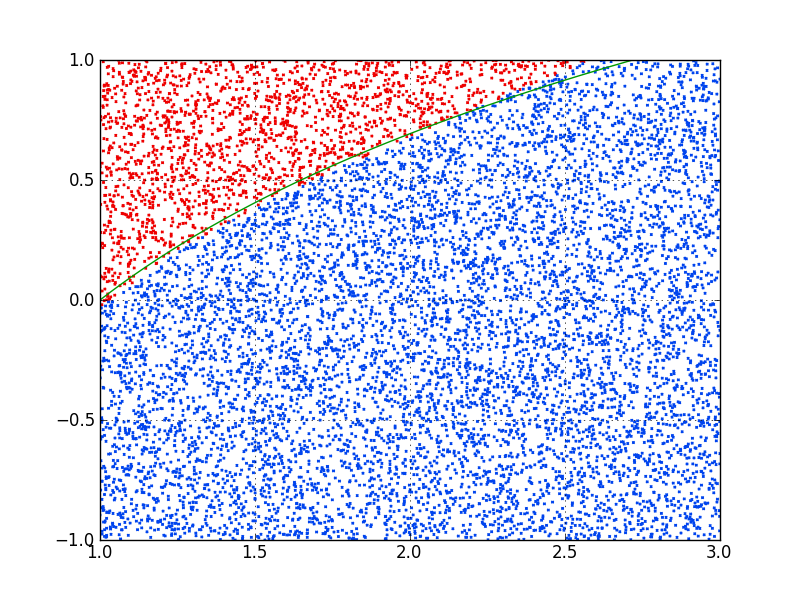
\includegraphics[scale=0.5]{test.png}\\ 

Compare this to the same function classified with a network with only one hidden layer comprised of 10 nodes: \\ 
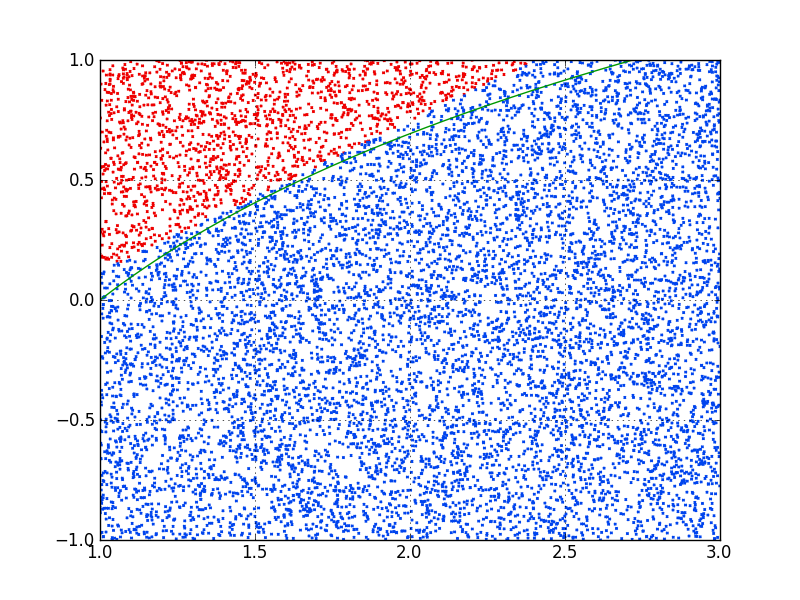
\includegraphics[scale=0.5]{test2.png}\\ 

Here's an example with the $x^2$ function, with 2 hidden layers, one of 3 nodes, and one of 2 nodes: \\ 
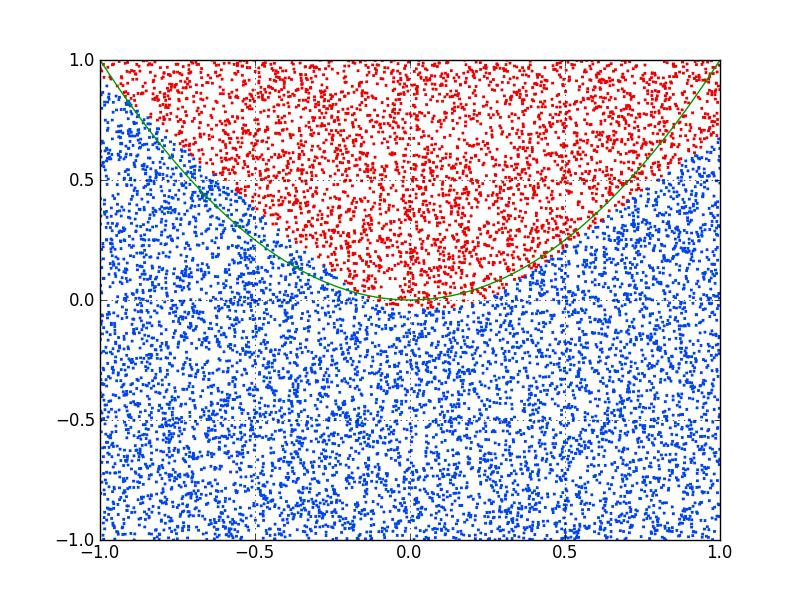
\includegraphics[scale=0.5]{test3.png}\\

And the same function, but with only one hidden layer of 3 nodes: \\ 
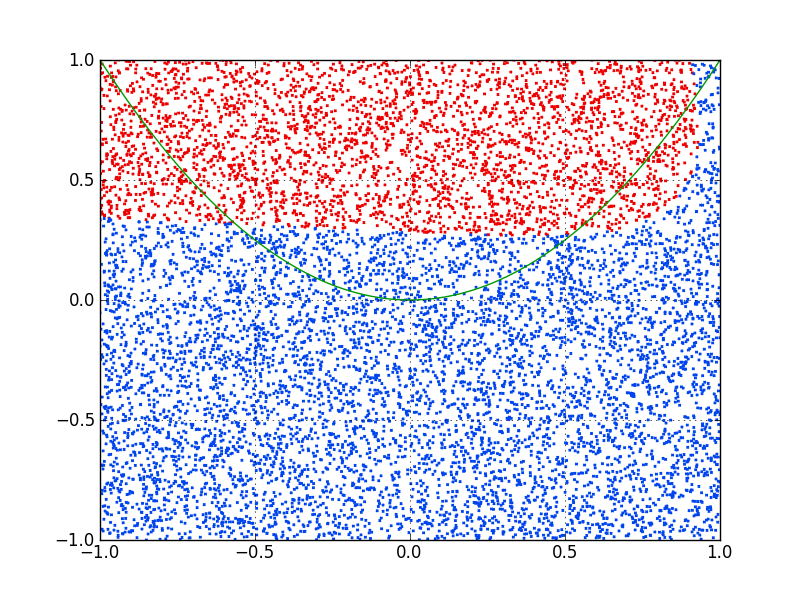
\includegraphics[scale=0.5]{test4.png}\\

And $\tanh(\pi x)$, with a hidden layer of 3 nodes, and one of 2: \\ 
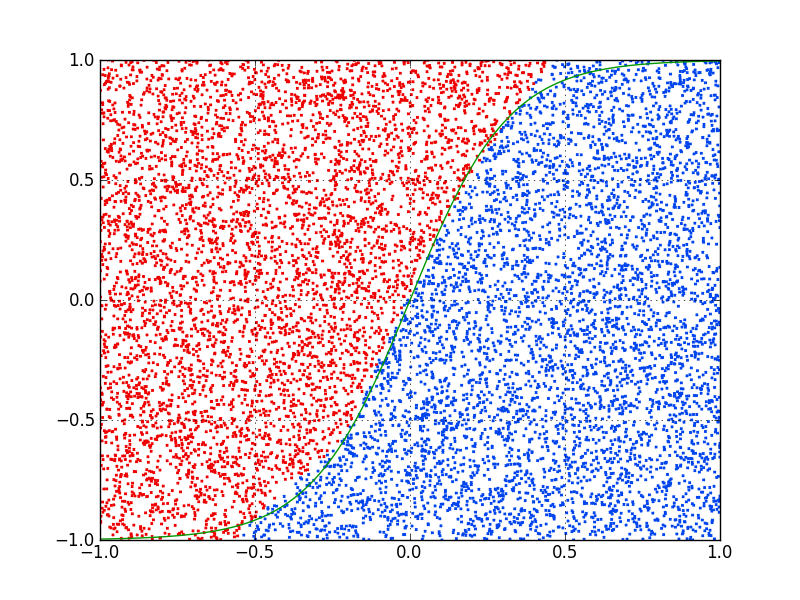
\includegraphics[scale=0.5]{test5.png}\\

Finally, $\cos(2 \pi x)$, with a hidden layer of 5 nodes, and one of 3 and 1000 epochs: \\ 
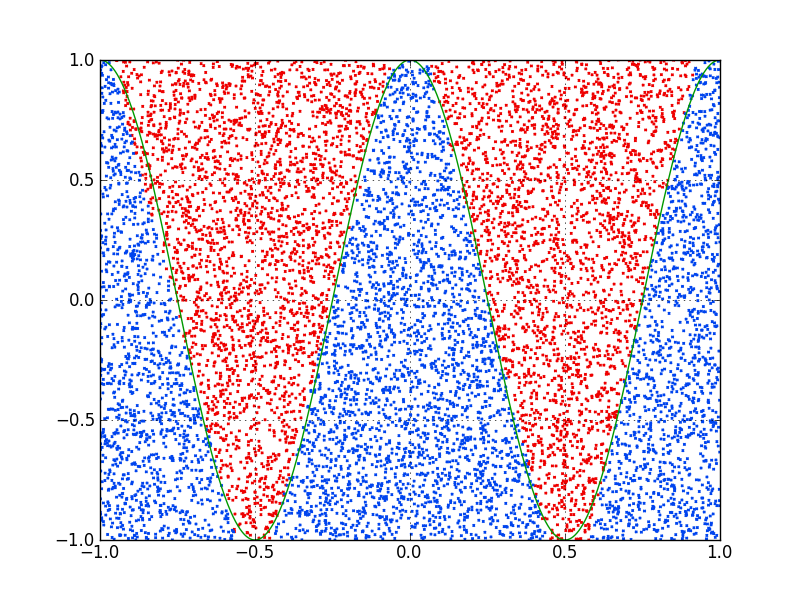
\includegraphics[scale=0.5]{test6.png}\\

Finally, $\frac{1}{2} \cos(2 \pi x) + \frac{1}{2} \cos(3 \pi x)$, with a hidden layer of 7 nodes, and one of 5 and 5000 epochs: \\ 
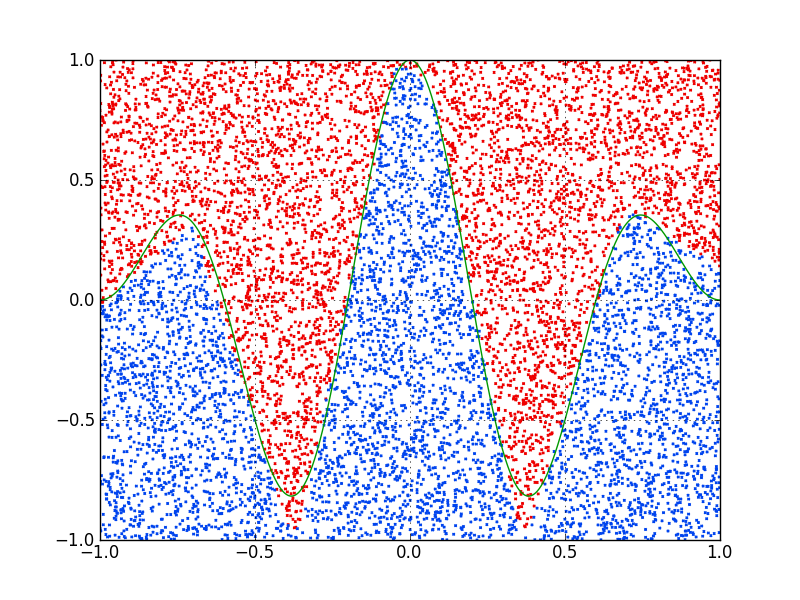
\includegraphics[scale=0.5]{test7.png}\\

With more training and more nodes, the networks become more precise.

\item[Examples] 
The various command-line options are documented by using the \emph{-h} flag. Below are some instructive and fun examples. 100 epoch examples takes around 5-10 seconds on a i5 CPU.
	\begin{enumerate}
		\item
			This creates and trains for 100 epochs a neural network with 2 input nodes (this is required), and two layers of 3 hidden nodes, and the single required output. The neural network is saved to nn.txt\\ \\
			|brains --function-spec "x**2" -t -s 'nn.txt' --epochs 100| \\ 
				|--nn-spec "2 5 3 1"|
		\item
			This loads the previously created neural network from the file nn.txt, and runs (default=1000) it on test data, plotting the points as well as the function, and saving the graphic to t.png. \\ \\
			|brains -l nn.txt --function-spec "x**2" --l-ylim 0 --test-png t.png|
		\item
			This trains and outputs graphs on both the testing and the training data. Note the moved x-axes; this is necessary to avoid a domain error for the log function. The default domain and range is (-1,1).\\ \\
			|brains --function-spec "math.log(x)" --l-xlim 1 --r-xlim 3 -t -s | \\ 
			|'nn2.txt' --epochs 1000 --nn-spec "2 5 1" --test-png test.png |\\ 
			|--training-png train.png|
		\item
			This runs the neural networked saved to nn2.txt on the given points, outputting the results of the neural network. \\ \\
			|brains -l nn2.txt -r "[[2,2],[1.5,2.3],[1.1,-0.5]]"|
	\end{enumerate}

\item[Notes]
It seems as though more layers indeed increases the resolution of the network. More epochs, as expected, is not always better, and more layers or nodes is not either. There is also great variation in accuracy at convergence with different initial weights. This makes sense given the existence of local optima that gradient descent tend towards, but I hadn't expected it to the degree I found it.

\item[Exploration]
I'd like to parallelize this algorithm, and try various brain damage and inter-layer connections. In addition, it would be useful to write the neural network in Haskell or C, and call it from the CLI |brains| for greatly increased performance, as well as ease of parallelization. 

\end{enumerate}
\end{document}